
\section{丰富与极丰富线丛}

现在我们来引入\trAmpleness。\trLineBundle{}的这条核心的「正性」（positivity）性质，将因许多各不相同的理由——几何的、代数的、拓扑的、计算的，等等——而被证明是重要的。

设 $\pi\colon X\to\Spec A$ 是一个\trMorphism，而 $\mathscr{L}$ 是 $X$ 上一个\trInvertibleSheaf。（$A$ 是\trField{}的情形，是最直接令人感兴趣的情形。）若 $X\cong\Proj S_\bullet$，其中 $S_\bullet$ 是 $A$ 上一个\trFinitelyGenerated{}、在次数 $1$ 处生成的\trGradedRing（\mbox{定义~4.5.6}），且 $\mathscr{L}\cong\OO_{\Proj S_\bullet}(1)$，我们就称 $\mathscr{L}$ 为\textbf{在 $A$ 上\trVeryAmple{}的}（very ample over $A$）、\textbf{$\pi$-\trVeryAmple{}的}（$\pi$-very ample）或\textbf{相对\trVeryAmple{}的}（relatively very ample）。当\trStructureMorphism{}从上下文来看是清楚的时，人们常径称\textbf{\trVeryAmple}。注意，\trVeryAmple\trLineBundle{}的存在性蕴含 $X$ 是\trProjective{}的。

\textbf{16.2.A.（容易但重要的练习：$A$ 上\trVeryAmple{}的等价定义）}\quad 设 $\pi\colon X\to\Spec A$ 是\trProper{}的，而 $\mathscr{L}$ 是 $X$ 上一个\trInvertibleSheaf。证明：$\mathscr{L}$ 是\trVeryAmple{}的，当且仅当存在有限多个\trGlobalSections{} $s_0,\dots,s_n$\footnote{原书此处作「$s_0,\dots s_n$」，省略号之后无逗号（同条展示式则作 $[s_0,\dots,s_n]$，有逗号），当为脱逗之误，径补。——译者注}，它们没有公共零点，使得\trMorphism
\[
[s_0,\dots,s_n]\colon X\longrightarrow\mathbb{P}^n_A
\]
是一个\trClosedEmbedding。

\textbf{16.2.B.（容易的练习：\trVeryAmple{}蕴含\trBasePointFree）}\quad 证明：\trProper{} $A$-\trScheme{}上一个\trVeryAmple{}的\trInvertibleSheaf{} $\mathscr{L}$ 必是\trBasePointFree{}的。换言之，证明：对该\trScheme{}上任意一点 $p$，都存在 $\mathscr{L}$ 的一个在 $p$ 处不消失的\trSection。

\textbf{16.2.C.（练习：\trVeryAmple{}$\otimes$\trBasePointFree{}的是\trVeryAmple{}的，从而\trVeryAmple{}$\otimes$\trVeryAmple{}的是\trVeryAmple{}的）}\quad 设 $\mathscr{L}$ 与 $\mathscr{M}$ 是\trProper{} $A$-\trScheme{} $X$ 上的两个\trInvertibleSheaf，$\mathscr{L}$ 在 $A$ 上\trVeryAmple{}，而 $\mathscr{M}$ \trBasePointFree。证明：$\mathscr{L}\otimes\mathscr{M}$ 是\trVeryAmple{}的。（提示：$\mathscr{L}$ 给出一个\trClosedEmbedding{} $X\hookrightarrow\mathbb{P}^m$，$\mathscr{M}$ 给出一个\trMorphism{} $X\to\mathbb{P}^n$。证明积映射 $X\to\mathbb{P}^m\times\mathbb{P}^n$ 是\trClosedEmbedding，做法是对 $X\to\mathbb{P}^m\times\mathbb{P}^n\to\mathbb{P}^m$ 用关于闭嵌入的\trCancellationTheorem~11.1.1。最后，考虑复合映射 $X\hookrightarrow\mathbb{P}^m\times\mathbb{P}^n\hookrightarrow\mathbb{P}^{mn+m+n}$，其中最后一个闭嵌入是\trSegre{}嵌入。）

\textbf{16.2.D.（练习：\trVeryAmple{}$\boxtimes$\trVeryAmple{}的是\trVeryAmple{}的；参\mbox{例~15.2.10}）}\quad 设 $X$ 与 $Y$ 是\trProper{} $A$-\trScheme，而 $\mathscr{L}$（相应地，$\mathscr{M}$）是 $X$（相应地，$Y$）上一个\trVeryAmple{}的\trInvertibleSheaf。若 $\pi_X\colon X\times_A Y\to X$ 与 $\pi_Y\colon X\times_A Y\to Y$ 是通常的\trProjection，证明：$\pi_X^*\mathscr{L}\otimes\pi_Y^*\mathscr{M}$（亦名 $\mathscr{L}\boxtimes\mathscr{M}$；见 \S15.2.10）在 $X\times_A Y$ 上是\trVeryAmple{}的。

\textbf{16.2.1.\ \trhDefinition{}。}\quad 我们称\trProper{} $A$-\trScheme{} $X$ 上的一个\trInvertibleSheaf{} $\mathscr{L}$ 为\textbf{在 $A$ 上\trAmple{}的}（ample over $A$）、或\textbf{$\pi$-\trAmple{}的}（$\pi$-ample；$\pi\colon X\to\Spec A$ 即\trStructureMorphism）、或\textbf{相对\trAmple{}的}（relatively ample），若下述诸等价条件之一成立。

\textbf{16.2.2.\ \trhTheorem{}。}\ ——\ \emph{设 $\pi\colon X\to\Spec A$ 是\trProper{}的，而 $\mathscr{L}$ 是 $X$ 上一个\trInvertibleSheaf。则以下诸条件等价。}

\underline{\emph{射影几何：}}

\emph{(a) 对某个 $\mathrm{N}>0$，$\mathscr{L}^{\otimes\mathrm{N}}$ 在 $A$ 上是\trVeryAmple{}的。}

\emph{(a') 对一切 $n\gg 0$，$\mathscr{L}^{\otimes n}$ 在 $A$ 上是\trVeryAmple{}的。}

\underline{\emph{整体生成：}}

\emph{(b) 对一切\trFiniteType{}的\trQCSheaf{} $\mathscr{F}$，存在某个 $n_0$，使得对 $n\ge n_0$，$\mathscr{F}\otimes\mathscr{L}^{\otimes n}$ 都是\trGloballyGenerated。}

\underline{\emph{拓扑：}}

\emph{(c) 当 $\mathrm{f}$ 跑遍 $\mathscr{L}^{\otimes n}$ 的全部\trGlobalSections（对一切 $n>0$），诸开子集 $X_{\mathrm{f}}=\{p\in X:\mathrm{f}(p)\neq 0\}$ 构成 $X$ 之拓扑的一组\trBase。}

\emph{(c') 当 $\mathrm{f}$ 跑遍 $\mathscr{L}^{\otimes n}$ 的诸\trGlobalSections（对一切 $n>0$），其中\trAffine{}的那些开子集 $X_{\mathrm{f}}$ 构成 $X$ 之拓扑的一组\trBase。}

\emph{(c'') 当 $\mathrm{f}$ 跑遍 $\mathscr{L}^{\otimes n}$ 的诸\trGlobalSections（对一切 $n>0$），其中\trAffine{}的那些开子集 $X_{\mathrm{f}}$ 覆盖 $X$。}

（\mbox{定理~16.2.2} 在「绝对」与「相对」两种设定下的变体，将分别由\mbox{定理~16.2.6} 与\mbox{定理~17.3.7} 给出。）

注意，$(b)$ 与 $(c)$--$(c'')$ 都不曾提及\trStructureMorphism{} $\pi$。我们日后（\mbox{定理~18.8.1}）将会遇到\trAmpleness{}的一个上同调判别法（归功于\trSerre）。\trKodaira{}嵌入定理（见如 [GH1, p.~181]）也在复范畴中给出\trAmpleness{}的一个判别法：若 $X$ 是一个\trCompact\trComplex\trManifold，则 $X$ 上一个\trInvertibleSheaf{} $\mathscr{L}$ 是\trAmple{}的，当且仅当它容许一个处处曲率为正的\trHermitianMetric{}（Hermitian metric）。

这些条件的种种不同风味，从某些侧面表明：\trAmpleness{}在不少方面都比\trVeryAmpleness{}表现得更规整。我们无证明地再提一条性质（「丰富性是族中的开条件」）：若 $\pi\colon X\to T$ 是一个有限表现的\trProper\trMorphism，而 $\mathscr{L}$ 是 $X$ 上一个\trInvertibleSheaf，则 $T$ 上那些使 $\mathscr{L}$ 在纤维上丰富的点构成 $T$ 的一个开子集。此外，在这个开子集上，$\mathscr{L}$ 在基底上是相对\trAmple{}的。我们不会用到这些事实（证明见 [Gr-EGA, IV$_3$, 9.6.4]），但它们值得知晓。

在着手\mbox{定理~16.2.2} 的证明之前，我们先给出几个示例性的应用。我们以指出下面这一事实开篇：$(a)$ 蕴含 $(b)$，便给出\trSerre{}定理~A（\mbox{定理~16.1.5}）。

\textbf{16.2.E.（重要的练习）}\quad 设 $\mathscr{L}$ 与 $\mathscr{M}$ 是\trProper{} $A$-\trScheme{} $X$ 上的两个\trInvertibleSheaf，而 $\mathscr{L}$ 是\trAmple{}的。证明：对 $n\gg 0$，$\mathscr{L}^{\otimes n}\otimes\mathscr{M}$ 是\trVeryAmple{}的。（提示：把 \mbox{定理~16.2.2} 的 $(a)$ 与 $(b)$ 都用上，再用\mbox{练习~16.2.C}。）

\textbf{16.2.F.（重要的练习）}\quad 证明：\trProjective{} $A$-\trScheme{} $X$ 上每个\trLineBundle{}都是两个\trVeryAmple\trLineBundle{}之差。更精确地说，对 $X$ 上任意\trInvertibleSheaf{} $\mathscr{L}$，我们都能找到两个\trVeryAmple{}的\trInvertibleSheaf{} $\mathscr{M}$ 与 $\mathscr{N}$，使得 $\mathscr{L}\cong\mathscr{M}\otimes\mathscr{N}^{\vee}$。（提示：用上一题。）

\textbf{16.2.G.（重要的练习：反复使用）}\quad 设 $\pi\colon X\to Y$ 是\trProper{} $A$-\trScheme{}之间的一个\trFinite\trMorphism，而 $\mathscr{L}$ 是 $Y$ 上一个\trAmple\trLineBundle。证明：$\pi^*\mathscr{L}$ 在 $X$ 上是\trAmple{}的。提示：用\mbox{定理~16.2.2}$(c'')$ 的判别法。（对已在 \S16.2.5 中读过绝对情形丰富性的读者附言：该结果在那个情形同样适用，也就是说，把「\trProper{} $A$-\trScheme」改成「概形」后原封不动。唯一还需要注意的是：$\mathscr{L}$ 在 $Y$ 上的\trAmpleness{}由定义蕴含 $Y$ 是\trQuasicompact{}的，并由\mbox{定理~16.2.6}(d) 蕴含 $Y$ 是\trSeparated{}的。该结果的一个相对版本出现在 \S17.3.6。它还可以进一步推广——把「$\pi$ 有限」换成「$\pi$ 拟仿射」（将在 \S17.3.11 中定义）——见 [Gr-EGA, II.5.1.12]。）

\textbf{16.2.H.（练习：\trAmple{}$\otimes$\trAmple{}的是\trAmple{}的，\trAmple{}$\otimes$\trBasePointFree{}的是\trAmple{}的）}\quad 设 $\mathscr{L}$ 与 $\mathscr{M}$ 是\trProper{} $A$-\trScheme{} $X$ 上的两个\trInvertibleSheaf，且 $\mathscr{L}$ 是\trAmple{}的。证明：若 $\mathscr{M}$ 是\trAmple{}的或\trBasePointFree{}的，则 $\mathscr{L}\otimes\mathscr{M}$ 是\trAmple{}的。

\textbf{16.2.I.（不太重要的练习：\trAmple{}$\boxtimes$\trAmple{}的是\trAmple{}的）}\quad 把\mbox{练习~16.2.D} 中的「\trVeryAmple」换成「\trAmple」后求解之。

\textbf{16.2.J.（练习：参\mbox{练习~12.3.C}）}\quad 设 $X$ 是一个\trProjective{} $k$-\trScheme，$\mathscr{L}$ 是 $X$ 上一个\trAmple\trLineBundle，$\mathscr{M}$ 是 $X$ 上一个\trLineBundle，而 $q_1,\dots,q_m$ 是 $X$ 的点（不必是闭点）。证明：对每个 $\mathrm{N}\gg 0$，都存在 $\mathscr{L}^{\otimes\mathrm{N}}\otimes\mathscr{M}$ 的一个在任何一个 $q_i$ 上都不消失的\trSection。（提示：若 $q_1$ 不在任何其余 $q_i$ 的闭包之中，则用\mbox{定理~16.2.2}(b) 的判别法，配合一个精挑细选的 $\mathscr{F}$，找出 $\mathscr{L}^{\otimes\mathrm{N}}\otimes\mathscr{M}$ 的一个在除 $q_1$ 外的全部 $q_i$ 上消失、却在 $q_1$ 处不消失的\trSection。）本练习主要在 $k$ 是有限域时有趣。你可以用它来解带星的\mbox{练习~18.4.L}（经由\mbox{练习~16.2.L}）；而在\mbox{命题~20.1.6} 的证明中它也将被用到（经由\mbox{练习~16.2.K}）。

\textbf{16.2.K.（练习）}\quad 设 $X$ 是一个\trProjective{} $k$-\trScheme，$\mathscr{M}$ 是 $X$ 上一个\trLineBundle，而 $q_1,\dots,q_m$ 是 $X$ 的点（不必是闭点）。证明：存在 $X$ 上不含 $q_1,\dots,q_m$ 的两个\trEffectiveCartierDivisor{} $\mathrm{D}_1$ 与 $\mathrm{D}_2$，使得 $\mathscr{M}\cong\OO(\mathrm{D}_1-\mathrm{D}_2)$。提示：\mbox{练习~16.2.J}。

\textbf{16.2.L.}\ \hard\ （练习）\quad 设 $C$ 是域 $k$ 上一条既约射影曲线\footnote{原书此处作「reduced projective projective curve」，其中 projective 一词重出，当为排印重文之误，径删。——译者注}，$\mathscr{L}$ 是 $C$ 上一个\trLineBundle，而 $q_1,\dots,q_m$ 是 $C$ 的闭点。利用\mbox{练习~16.2.J}，证明我们可以把 $\mathscr{L}$ 写成 $\OO(\sum n_jp_j)$ 的形式，其中诸 $p_j$ 是与诸 $q_i$ 互异的\trRegular{}点。提示：利用「$C$ 的非正则点构成一个有限集」（\S13.5.10）这一事实。把 $\mathscr{L}$ 写成两个\trVeryAmple\trLineBundle{}之差。

\textbf{16.2.3.}\ \emph{\mbox{定理~16.2.2} 在 $X$ 为\trNoether{}情形时的证明。}\quad 诺特假设只在证明中的一个点处被用到，我们将解释如何把它们去掉。

\begin{figure}[htbp]
\centering
\begin{tikzcd}[row sep=3.4em, column sep=2.6em]
&& (a)\ar[dll] && (a')\ar[ll,"\text{显然}"'] \\
(c)\ar[rr,bend right] && (c')\ar[ll,bend right,"\text{显然}"']\ar[rr,"\text{显然}"] && (c'')\ar[ull,"\text{较难}"']\ar[dll,"\text{较难}"] \\
&& (b)\ar[ull] &&
\end{tikzcd}
\caption{\mbox{定理~16.2.2} 之证明（最后一步之前）的结构。（依原书手绘图重绘。）}\label{fig:ample-proof-structure}
\end{figure}

我们大致按从最容易到最困难的顺序来处理各条蕴含。显然，$(a')$ 蕴含 $(a)$，而 $(c')$ 同时蕴含 $(c)$ 与 $(c'')$。

我们现在证明 $(c)$ 蕴含 $(c')$。设 $p$ 是 $X$ 的开子集 $\mathrm{U}$ 中的一点。我们要找的是一个含 $p$ 且含于 $\mathrm{U}$ 的\emph{\trAffine}的 $X_{\mathrm{f}}$。经收缩 $\mathrm{U}$，不妨设 $\mathrm{U}$ 是\trAffine{}的。由 $(c)$，$\mathrm{U}$ 含有某个含 $p$ 的 $X_{\mathrm{f}}$。但这个 $X_{\mathrm{f}}$ 是\trAffine{}的，因为它是\trLineBundle{}在某个\trAffineScheme{}上的一个截面的\trVanishingSet{}的\trComplement（\mbox{练习~8.3.E}），于是 $(c')$ 成立。注意以备后用：$(c)$ 与 $(c')$ 的等价性并不需要固有性假设。

我们接着证明 $(a)$ 蕴含 $(c)$。我们用 $\mathscr{L}$ 的某个幂将 $X$ 嵌入\trProjectiveSpace。给定一个\trClosedSubset{} $Z\subset X$，以及\trComplement{} $X\setminus Z$ 中的一点 $p$，我们要找的是某个 $\mathscr{L}^{\otimes\mathrm{N}}$ 的一个在 $Z$ 上消失、而在 $p$ 处不消失的\trSection。这样的截面的存在性由 $V(I(Z))=Z$（\mbox{练习~4.5.K}(c)）这一事实得到：$I(Z)$ 中存在某个（\trHomogeneous{}的）元素不在 $p$ 上消失。（这也顺带证明了 $(a)$ 蕴含 $(c')$，但我们用不着它。）

我们接着证明 $(b)$ 蕴含 $(c)$。设 $p$ 是 $X$ 的开子集 $\mathrm{U}$ 中的一点。我们要找的是 $\mathscr{L}^{\otimes\mathrm{N}}$ 的一个在 $p$ 处不消失、却在 $X\setminus\mathrm{U}$ 上消失的\trSection。

\begin{figure}[htbp]
\centering
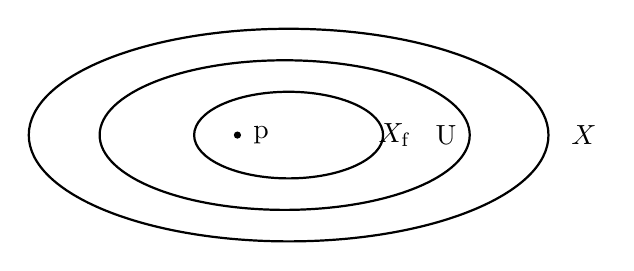
\begin{tikzpicture}[line width=0.8pt]
  \draw (0.2,0) ellipse (3.3 and 1.35);
  \draw (0.15,0) ellipse (2.35 and 0.95);
  \draw (0.2,0) ellipse (1.2 and 0.55);
  \fill (-0.45,0) circle (1.3pt);
  \node[anchor=west] at (-0.38,0) {$\mathrm{p}$};
  \node at (1.55,0) {$X_{\mathrm{f}}$};
  \node at (2.2,0) {$\mathrm{U}$};
  \node at (3.95,0) {$X$};
\end{tikzpicture}
\caption{\mbox{定理~16.2.2} 证明的直观辅助图。（依原书手绘图重绘。）}\label{fig:ample-visual-aid}
\end{figure}

令 $\mathscr{I}$ 为在 $X\setminus\mathrm{U}$ 上消失的那些函数所成的理想层（即以既约结构把 $X\setminus\mathrm{U}$ 割出来的那个\trQC{}理想层）。由于 $X$ 是\trNoether{}的，$\mathscr{I}$ 是\trFiniteType{}的，于是由 $(b)$，对某个 $\mathrm{N}$，$\mathscr{I}\otimes\mathscr{L}^{\otimes\mathrm{N}}$ 由\trGlobalSections{}生成，从而它有一个在 $p$ 处不消失的\trGlobalSections。（\emph{诺特附记}：这是整个论证中唯一用到诺特假设的地方。这些假设可以按如下方式去掉。证明：对一个\trQuasicompact\trQuasiSeparated{}概形，每个理想层都由其\trFiniteType{}的\trSubidealSheaf{}生成。事实上，\trQuasicompact\trQuasiSeparated{}概形上的任何\trQCSheaf{}都是它的\trFiniteType{}的\trQC{}子层之并。这件事可以徒手证明，是一道合用却困难的练习；例如见 [Stacks, tag~01PJ]。这些\trFiniteType{}理想层当中有一个在 $p$ 处不消失；拿它来顶替 $\mathscr{I}$ 即可。）

我们现在不得不开始更卖力地干活了。

我们接着证明 $(c'')$ 蕴含 $(b)$。

我们希望证明：对 $n\gg 0$，$\mathscr{F}\otimes\mathscr{L}^{\otimes n}$ 都是\trGloballyGenerated。我们先来证明 $(c'')$ 蕴含「对某个 $\mathrm{N}>0$，$\mathscr{L}^{\otimes\mathrm{N}}$ 是\trGloballyGenerated」，做法如下。利用 $X$ 的\trQuasicompactness，选出有限多个\trAffine{}的 $X_{\mathrm{f}_1},\dots,X_{\mathrm{f}_n}$ 覆盖 $X$，其中 $\mathrm{f}_i\in\Gamma(X,\mathscr{L}^{\otimes\mathrm{N}_i})$。把 $\mathrm{f}_i$ 换成 $\mathrm{f}_i^{\otimes(\prod_j\mathrm{N}_j)/\mathrm{N}_i}$，便可假定它们都是 $\mathscr{L}$ 的\emph{同一个}幂 $\mathscr{L}^{\otimes\mathrm{N}}$ 的截面（取 $\mathrm{N}=\prod_j\mathrm{N}_j$）。于是 $\mathscr{L}^{\otimes\mathrm{N}}$ 由这些\trGlobalSections{}生成。

我们接着证明：只需对一切\trFiniteType{}的\trQCSheaf{} $\mathscr{F}$ 证明「$\mathscr{F}\otimes\mathscr{L}^{\otimes m\mathrm{N}}$ 在 $m\gg 0$ 时是\trGloballyGenerated」就足够了。因为一旦知道这一点，便可把它施用于 $\mathscr{F}$，$\mathscr{F}\otimes\mathscr{L}^{\vee}$，…，$\mathscr{F}\otimes\mathscr{L}^{\otimes(\mathrm{N}-1)}$（共有限多次），结论随之而来。出于这一理由，我们可以把 $\mathscr{L}$ 换成 $\mathscr{L}^{\otimes\mathrm{N}}$。换言之，为证 $(c'')$ 蕴含 $(b)$，我们还可以添上「$\mathscr{L}$ 是\trGloballyGenerated」这条附加假设。

对每个闭点 $p$，利用 $(c'')$ 选一个形如 $X_{\mathrm{f}}$ 的\trAffine\trOpen\trNeighborhood。于是 $\mathscr{F}|_{X_{\mathrm{f}}}$ 由有限多个\trGlobalSections{}生成（容易的\mbox{练习~16.1.B}——$\Spec A$ 上一个\trFiniteType{}的\trQCSheaf{}对应于一个\trFinitelyGenerated{}的 $A$-\trModule）。由\mbox{练习~15.4.N}，这些生成元中的每一个都可表示成 $\mathscr{F}\otimes\mathscr{L}^{\otimes M(p)}$ 在 $X$ 上的一个\trSection{}除以 $\mathrm{f}^{M(p)}$ 的商。（注意：对每个 $p$，可以取定单独一个 $M(p)$。）于是 $\mathscr{F}\otimes\mathscr{L}^{\otimes M(p)}$ 在 $p$ 处由有限多个\trGlobalSections{}生成。由\mbox{练习~16.1.D}(b)，$\mathscr{F}\otimes\mathscr{L}^{\otimes M(p)}$ 在 $p$ 的某个\trOpen\trNeighborhood{} $\mathrm{U}_p$ 中的所有点处都整体生成。由于 $\mathscr{L}$ 也整体生成，这蕴含：对一切 $M'\ge M(p)$，$\mathscr{F}\otimes\mathscr{L}^{\otimes M'}$ 在 $\mathrm{U}_p$ 的一切点处都整体生成（对照容易的\mbox{练习~16.1.C}）。由 $X$ 的\trQuasicompactness，这些 $\mathrm{U}_p$ 中有限多个便覆盖 $X$，于是（取诸 $M(p)$ 的最大者）证毕。

我们的倒数第二步是证明 $(c'')$ 蕴含 $(a)$。设 $(c'')$ 成立。目标便是找到某个 $\mathscr{L}^{\otimes\mathrm{N}}$ 的若干截面，把 $X$ 嵌入\trProjectiveSpace。选取（拟紧的）$X$ 的一个由 $n$ 个\trAffine\trOpenSubset{}组成的覆盖 $X_{a_1},\dots,X_{a_n}$，其中 $a_1,\dots,a_n$ 都是 $\mathscr{L}$ 的幂的截面。把每个截面换成适当的幂之后，便可假定它们都是 $\mathscr{L}$ 的\emph{同一个}幂（设为 $\mathscr{L}^{\otimes\mathrm{N}}$）的截面。设 $X_{a_i}=\Spec A_i$，其中（利用 $\pi$ 为\trFiniteType{}这一事实）$A_i=A[a_{i_1},\dots,a_{i_j}]/I_i$\footnote{原书此处作「$A_i=\Spec A[a_{i_1},\dots,a_{i_j}]/I_i$」，其中的 $\Spec$ 当系衍文（其前已设 $X_{a_i}=\Spec A_i$，$A_i$ 应为环），径删。——译者注}。由\mbox{练习~15.4.N}，每个 $a_{ij}$ 都形如 $s_{ij}/a_i^{m_{ij}}$，其中 $s_{ij}\in\Gamma(X,\mathscr{L}^{\otimes\mathrm{N}m_{ij}})$（对某个 $m_{ij}$）。令 $m=\max_{i,j}m_{ij}$。于是对每一对 $i,j$，$a_{ij}=(s_{ij}a_i^{m-m_{ij}})/a_i^{m}$。为方便计，令 $b_i=a_i^{m}$，$b_{ij}=s_{ij}a_i^{m-m_{ij}}$；这些都是 $\mathscr{L}^{\otimes m\mathrm{N}}$ 的\trGlobalSections。现在考虑由诸 $b_i$ 与诸 $b_{ij}$ 生成的\trLinearSystem。由于 $\mathrm{D}(b_i)=X_{a_i}$ 覆盖 $X$，这个\trLinearSystem{}是\trBasePointFree{}的，从而（由\mbox{练习~15.2.A}）给出一个到 $\mathbb{P}^{\mathrm{Q}}$ 的\trMorphism（其中 $\mathrm{Q}=\#b_i+\#b_{ij}-1$）。令 $x_1,\dots,x_n,\dots,x_{ij},\dots$ 为 $\mathbb{P}^{\mathrm{Q}}$ 上的射影\trCoordinate（于是 $\mathrm{f}^*x_i=b_i$，而 $\mathrm{f}^*x_{ij}=b_{ij}$）。于是诸\trAffineScheme{}之间的态射 $X_{a_i}\to\mathrm{D}(x_i)$ 都是\trClosedEmbedding，因为相伴的环映射是满射（$A_i$ 的\trGenerator{} $a_{ij}$ 正是 $x_{ij}/x_i$ 的\trImage）。

至此，我们为日后记下这么一件事：我们已经证明了下面这个结论。若 $X\to\Spec A$ 是\trFiniteType{}的，而 $\mathscr{L}$ 满足 $(c'')$，则 $X$ 是到某个\trProjective{} $A$-\trScheme{}的一个\trLocallyClosedEmbedding。（我们没有用到分离性。）我们用\mbox{练习~11.4.C}（「固有的像是固有的」）来断结 $(c'')$ 蕴含 $(a)$ 的证明：这个局部闭嵌入到射影 $A$-概形之中的\trImage{}实际上是闭的，故 $X$ 是一个\trProjective{} $A$-\trScheme。（你可看得出为什么带闭\trImage{}的\trLocallyClosedEmbedding{}实际上是\trClosedEmbedding？）

最后，我们指出 $(a)$ 与 $(b)$ 合起来蕴含 $(a')$：若 $\mathscr{L}^{\otimes\mathrm{N}}$ 是\trVeryAmple{}的（由 $(a)$），而 $\mathscr{L}^{\otimes n}$ 对 $n\ge n_0$ 是\trBasePointFree{}的（由 $(b)$），则由\mbox{练习~16.2.C}，$\mathscr{L}^{\otimes n}$ 对 $n\ge n_0+\mathrm{N}$ 是\trVeryAmple{}的。\hfill$\square$

\textbf{16.2.4.}\ \extrahard\ \emph{\trSemiample\trLineBundle。}\quad 正如一个\trInvertibleSheaf{}在它的某个张量幂是\trVeryAmple{}的时便是\trAmple{}的，若一个\trInvertibleSheaf{} $\mathscr{L}$ 的某个张量幂是\trBasePointFree{}的，我们就称 $\mathscr{L}$ 为\textbf{\trSemiample{}的}（semiample）。（解说：$\mathscr{L}$ 是\trAmple{}的，是说它的某个幂给出一个到\trProjectiveSpace{}的\trClosedEmbedding；$\mathscr{L}$ 是\trSemiample{}的，是说它的某个幂只给出一个到\trProjectiveSpace{}的\emph{\trMorphism}。）我们不会用到这个概念。

\textbf{16.2.5.}\ \hard\ \textbf{绝对情形下的\trAmpleness。}\quad （本节内容日后不会被我们以任何严肃的方式用到。）注意，整体生成已然是一个绝对性的概念，也就是说，它对概形上的一个\trQCSheaf{}有定义，不涉及任何\trMorphism。对\mbox{定理~16.2.2} 的证明稍加检视便知，\trAmpleness{}同样可以在一种绝对的情形下解释。我们把这件事说精确。设 $\mathscr{L}$ 是一个\emph{\trQuasicompact}的概形 $X$ 上的\trInvertibleSheaf。我们称 $\mathscr{L}$ 为\textbf{\trAmple{}的}（ample），若当 $\mathrm{f}$ 跑遍 $\mathscr{L}^{\otimes n}$ 的诸\trSection{}（$n>0$），诸开子集 $X_{\mathrm{f}}=\{p\in X:\mathrm{f}(p)\neq 0\}$ 构成 $X$ 之拓扑的一组\trBase。（我们强调，$X$ 的拟紧性是「$\mathscr{L}$ 是\trAmple{}的」这一条件的一部分。）例如：(i) 若 $X$ 是一个\trAffineScheme，则每个\trInvertibleSheaf{}都是\trAmple{}的；(ii) 若 $X$ 是一个\trProjective{} $A$-\trScheme，则 $\OO(1)$ 是\trAmple{}的。

\textbf{16.2.M.（容易的练习：绝对丰富性的性质）}\quad

（a）取定一个正整数 $n$。证明：$\mathscr{L}$ 是\trAmple{}的，当且仅当 $\mathscr{L}^{\otimes n}$ 是\trAmple{}的。

（b）证明：若 $Z\hookrightarrow X$ 是一个\trClosedEmbedding，而 $\mathscr{L}$ 在 $X$ 上是\trAmple{}的，则 $\mathscr{L}|_Z$ 在 $Z$ 上是\trAmple{}的。

下面这条结果会让你对丰富性的行为方式有几分感觉。我们不会用到它，因而略去其证明（证明见 [Stacks, tag~01Q3]）。不过，该证明的许多部分与\mbox{定理~16.2.2} 中相应的论证如出一辙（或为其推广）。诸陈述的标号编排与\mbox{定理~16.2.2} 中诸陈述的标号编排平行一致。

\textbf{16.2.6.\ \trhTheorem{}（对照\mbox{定理~16.2.2}）。}\ ——\ \emph{设 $\mathscr{L}$ 是一个\trQuasicompact{}概形 $X$ 上的\trInvertibleSheaf。则以下诸条件等价。}

\emph{(b) $X$ 是\trQuasiSeparated{}的，且对每个\trFiniteType{}的\trQCSheaf{} $\mathscr{F}$，存在某个 $n_0$，使得对 $n\ge n_0$，$\mathscr{F}\otimes\mathscr{L}^{\otimes n}$ 都是\trGloballyGenerated。}

\emph{(c) 当 $\mathrm{f}$ 跑遍 $\mathscr{L}^{\otimes n}$ 的诸\trGlobalSections（$n>0$），诸开子集 $X_{\mathrm{f}}=\{p\in X:\mathrm{f}(p)\neq 0\}$ 构成 $X$ 之拓扑的一组\trBase（也就是说，$\mathscr{L}$ 是\trAmple{}的）。}

\emph{(c') 当 $\mathrm{f}$ 跑遍 $\mathscr{L}^{\otimes n}$ 的诸\trGlobalSections（$n>0$），其中\trAffine{}的那些开子集 $X_{\mathrm{f}}$ 构成 $X$ 之拓扑的一组\trBase。}

\emph{(c'') 当 $\mathrm{f}$ 跑遍 $\mathscr{L}^{\otimes n}$ 的诸\trGlobalSections（$n>0$），其中\trAffine{}的那些开子集 $X_{\mathrm{f}}$ 覆盖 $X$。}

\emph{(d) 令 $S_\bullet$ 为分次环 $\oplus_{n\ge 0}\Gamma(X,\mathscr{L}^{\otimes n})$。则诸开集 $X_{\mathrm{f}}$（其中 $\mathrm{f}\in S_+$ 是正次数的\trHomogeneous{}元素）覆盖 $X$，且相伴的映射 $X\to\Proj S_\bullet$ 是一个\trOpenEmbedding。（警告：$S_\bullet$ 未必\trFinitelyGenerated，而 $\Proj S_\bullet$ 也未必是\trFiniteType{}的。）}

$(d)$ 部分蕴含 $X$ 是\trSeparated{}的（从而是\trQuasiSeparated{}的）。

\textbf{16.2.7.}\ \hard\ \textbf{把整体生成、无基点性与丰富性搬运到相对情形。}\quad 这些观念都可以被「相对化」。我们本可以现在就动手做这件事，但我们将等到 \S17.3.5——届时我们将已经定义了\trProjective\trMorphism{}的观念，从而也定义了「相对\trVeryAmple」的\trLineBundle——再做。
